% =============================================================================
% mazoti.ma -- The mathematics of Moroccan fuel prices
% Build:  cd docs/latex && python3 make_examples.py (from repo root, see Appendix D)
%         pdflatex mazoti_theory.tex  (run twice)
% All numbers in tables and plots come from generated/ (produced by make_examples.py).
% =============================================================================
\documentclass[11pt,a4paper]{article}

\usepackage[T1]{fontenc}
\usepackage[utf8]{inputenc}
\usepackage{lmodern}
\usepackage[margin=2.5cm]{geometry}
\usepackage{microtype}
\usepackage{amsmath,amssymb,amsthm}
\usepackage{booktabs,longtable,array}
\usepackage{enumitem}
\usepackage{xcolor}
\usepackage{graphicx}
\usepackage{float}
\usepackage{tikz}
\usetikzlibrary{positioning,arrows.meta,calc,shapes.geometric}
\usepackage{pgfplots}
\pgfplotsset{compat=1.16}
\usepackage[most]{tcolorbox}
\usepackage[colorlinks=true,linkcolor=blue!50!black,citecolor=blue!50!black,urlcolor=blue!50!black]{hyperref}

\setlength{\parindent}{0pt}
\setlength{\parskip}{0.6em}
\renewcommand{\arraystretch}{1.15}

% ---- evidence tags --------------------------------------------------------
\newcommand{\tagV}{\textsuperscript{\textcolor{green!50!black}{\textsf{\scriptsize[V]}}}}
\newcommand{\tagS}{\textsuperscript{\textcolor{orange!80!black}{\textsf{\scriptsize[S]}}}}
\newcommand{\tagQ}{\textsuperscript{\textcolor{red!70!black}{\textsf{\scriptsize[?]}}}}

% ---- boxes ----------------------------------------------------------------
\newtcolorbox{intuition}{colback=blue!4,colframe=blue!55!black,fonttitle=\bfseries,
  title=Intuition,breakable,boxrule=0.6pt,left=6pt,right=6pt}
\newtcolorbox{warning}{colback=red!4,colframe=red!60!black,fonttitle=\bfseries,
  title=Warning,breakable,boxrule=0.6pt,left=6pt,right=6pt}
\newtcolorbox{keyidea}{colback=green!4,colframe=green!45!black,fonttitle=\bfseries,
  title=Key idea,breakable,boxrule=0.6pt,left=6pt,right=6pt}
\newtcolorbox{worked}[1]{colback=gray!6,colframe=gray!60!black,fonttitle=\bfseries,
  title={Worked example: #1},breakable,boxrule=0.6pt,left=6pt,right=6pt}

\theoremstyle{definition}
\newtheorem{definition}{Definition}[section]

% ---- shorthand ------------------------------------------------------------
\newcommand{\MADL}{\text{MAD/L}}
\newcommand{\PT}{\mathrm{PT}}
\newcommand{\AI}{\mathrm{AI}}
\newcommand{\E}{\mathbb{E}}
\newcommand{\ind}{\mathbf{1}}

\title{\textbf{How Moroccan fuel prices work,\\ and how to measure them}\\[0.4em]
\large The mathematics behind mazoti.ma}
\author{Prepared with Claude for the mazoti.ma project}
\date{Version 0.1 --- 18 November 2026}

\begin{document}
\maketitle

\begin{abstract}
\noindent
This document explains, from first principles, the theory we will use to track Moroccan
pump prices and compare them with what the fuel costs to buy. It covers three things:
(i)~the \emph{structure} of a pump price (what it is made of and how to check that against
published figures); (ii)~the \emph{dynamics} (how fast and how fully world price changes reach
the pump, and whether rises and falls are treated alike); and (iii)~the \emph{statistics and
uncertainty} needed to say anything defensible about such questions with limited data.
Every table and figure is generated by code in the repository, so the text cannot drift from the
numbers. No prior knowledge of econometrics is assumed; derivations are collected in
Appendix~B and exercises with solutions in Appendix~C.
\end{abstract}

\tableofcontents
\newpage

% =============================================================================
\section*{How to read this document}
\addcontentsline{toc}{section}{How to read this document}

Each idea appears in up to three layers. \textbf{Intuition} boxes give the plain-language
picture. The main text gives the equations. \textbf{Worked examples} use numbers you can
check by hand. Warnings flag places where a careless reading gives a wrong or unfair
conclusion. Skip the equations on a first pass if you wish; the boxes alone tell the story.

Facts about Morocco carry an evidence tag, because much of what is public comes through the
press rather than primary documents:
\begin{center}
\begin{tabular}{cl}
\tagV & \textbf{Verified}: checked in a primary document (here, mainly the Competition Council reports)\\
\tagS & \textbf{Secondary}: reported by the press; primary text not yet checked\\
\tagQ & \textbf{To verify}: an assumption or a figure recalled but not yet checked
\end{tabular}
\end{center}

Amounts are in dirhams (MAD), volumes in litres (L), mass in tonnes (t). Two products are
considered: \emph{gasoil} (diesel) and \emph{SSP} (super sans plomb, 95-octane gasoline).

% =============================================================================
\part{The problem}

\section{What are we trying to find out?}

The public sees one number: the price on the pump. Behind it are four separate questions.

\begin{enumerate}[label=\textbf{Q\arabic*.},leftmargin=3em]
\item \textbf{Structure.} Of each dirham paid at the pump, how much is the cost of the fuel on
  the world market, how much is tax, and how much is margin for distributors and stations?
\item \textbf{Speed and completeness.} When the world cost changes, how quickly and how fully does the
  pump price follow?
\item \textbf{Symmetry.} Is the response the same when the cost rises as when it falls?
\item \textbf{Confidence.} How sure can we be, given that the true purchase costs of
  distributors are not public?
\end{enumerate}

Answering them requires more than putting the oil price and the pump price on one chart.

\begin{intuition}
Comparing the pump price with the price of a barrel of crude is like comparing a restaurant
bill with the price of flour. The pump price follows the price of \emph{refined products}
(diesel and gasoline), which can move quite differently from crude. It also includes taxes
that do not move at all with oil prices, is measured in litres rather than barrels or tonnes,
is paid in dirhams while the world quotes dollars, and is only revised every two weeks.
Each of these has to be handled before any comparison means anything.
\end{intuition}

\subsection*{A puzzle to keep in mind}

In autumn 2026 the press reports gasoil priced \emph{above} SSP at the pump (about 16.90 versus
15.50~MAD/L on 1~November)\tagS, the reverse of the usual order. Gasoil carries a lower fixed
tax than SSP, so the inversion means the pre-tax cost of diesel must be much higher than that of
gasoline. Section~\ref{sec:puzzle} turns this into a number we can test. Good theory makes a
puzzle like this a calculation rather than a debate.

\section{The institutional background}

\begin{itemize}
\item Morocco liberalised fuel prices on 1~December 2015; before then the state set them by a
  formula\tagS. Distributors now choose their prices and revise them on the 1st and 16th of
  each month\tagS.
\item Morocco imports all its refined products since the Samir refinery stopped\tagS. Pump prices
  follow refined-product quotations (``Platts'' quotations), with the Amsterdam--Rotterdam--Antwerp
  (ARA) hub as a main reference\tagV, not crude oil directly.
\item Two taxes apply\tagS: the \textbf{TIC} (\emph{taxe int\'erieure de consommation}), a fixed
  amount per litre collected at import, and \textbf{VAT} at 10\%, applied to the whole value
  including the TIC.
\item The Competition Council (CC) found anticompetitive practices among nine distributors and,
  on 23~November 2023, concluded settlements totalling 1.84 billion MAD with behavioural
  commitments\tagS. It now publishes quarterly follow-up reports; the Q4~2025 report is the
  ninth\tagV.
\end{itemize}

What the CC reports for nine distributors, as quarterly averages in MAD/L\tagV: the CIF
quotation, the purchase cost, the \emph{cession price} (the price charged by a distributor to
partner stations, before VAT), the pump price, and gross margins. It calls its CIF series
``indicative and theoretical'', not equal to actual procurement costs\tagV. Its reports appear
four to seven months after the quarter ends. Most of the project rests on two consequences:

\begin{keyidea}
\begin{enumerate}[leftmargin=1.5em]
\item The CC tables are our only ground truth; our model must reproduce them before we trust
  it anywhere else.
\item Because of the delay, anything we show for \emph{today} is model-based, and the screen must
  always say which numbers are observed, CC-reported or model-implied.
\end{enumerate}
\end{keyidea}

\subsection{The map of the approach}

\begin{figure}[H]
\centering
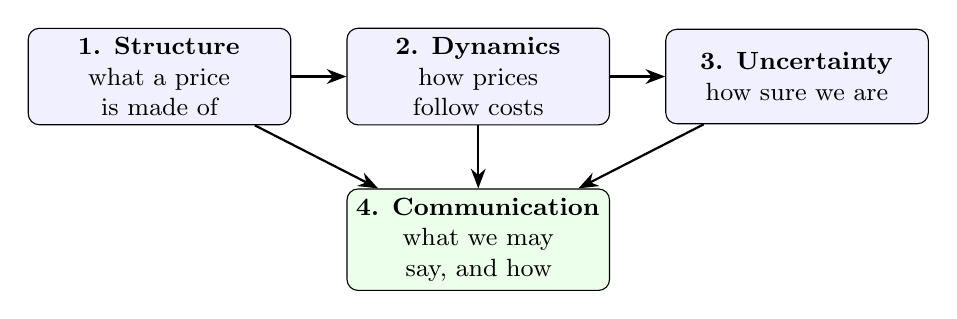
\begin{tikzpicture}[
  layer/.style={draw, rounded corners, align=center, minimum height=1.2cm, text width=3.1cm,
                font=\small, fill=blue!6},
  arr/.style={-{Stealth[length=2.5mm]}, thick}]
  \node[layer] (a) {\textbf{1. Structure}\\ what a price is made of};
  \node[layer, right=7mm of a] (b) {\textbf{2. Dynamics}\\ how prices follow costs};
  \node[layer, right=7mm of b] (c) {\textbf{3. Uncertainty}\\ how sure we are};
  \node[layer, below=8mm of b, fill=green!8] (d) {\textbf{4. Communication}\\ what we may say, and how};
  \draw[arr] (a)--(b); \draw[arr] (b)--(c); \draw[arr] (a)--(d); \draw[arr] (b)--(d); \draw[arr] (c)--(d);
\end{tikzpicture}
\caption{The four layers. Parts~II--VII develop layers 1--3; Part~VIII is about layer 4.}
\end{figure}

% =============================================================================
\part{Price structure}

\section{From a quotation to a price per litre}

World quotations for refined products are in \emph{US dollars per tonne} (USD/t). Pump prices are
in \emph{dirhams per litre}. The conversion needs the exchange rate $X$ (MAD per USD) and the
density $d$ (kg per litre), since a tonne of fuel holds $1000/d$ litres.

\begin{definition}[CIF cost per litre]
For a quotation $Q$ (USD/t),
\begin{equation}\label{eq:unit}
c \;=\; Q \cdot X \cdot \frac{d}{1000}\qquad [\MADL].
\end{equation}
\end{definition}
``CIF'' means cost, insurance and freight: the price delivered to the Moroccan port, before
taxes. Typical densities are about 0.84~kg/L for diesel and 0.745~kg/L for 95-octane
gasoline\tagQ. The CC does not state the factor it uses, so $d$ is a calibration parameter.

\begin{worked}{unit conversion}
$Q=700$~USD/t, $X=9.0$~MAD/USD (a round illustrative rate, not a market figure), $d=0.84$:
\[
c = 700 \times 9.0 \times \frac{0.84}{1000} = 5.292~\MADL .
\]
Check by reasoning: 1 tonne is about $1000/0.84 \approx 1190$~L, and $700\times 9 = 6300$~MAD per tonne,
so $6300/1190 \approx 5.29$~MAD/L.
\end{worked}

\begin{warning}
The density matters for the \emph{level} of $c$ but not for pass-through \emph{ratios}: if $d$ is
wrong by 2\%, every $c$ is off by 2\%, so $\Delta c/\Delta P$ is off by the same 2\% for all periods
and the shape of the series is unchanged. It matters when we compare the level of $c$ to the CC's
CIF series.
\end{warning}

\section{The chain: cost, margins, taxes}

\begin{figure}[H]
\centering
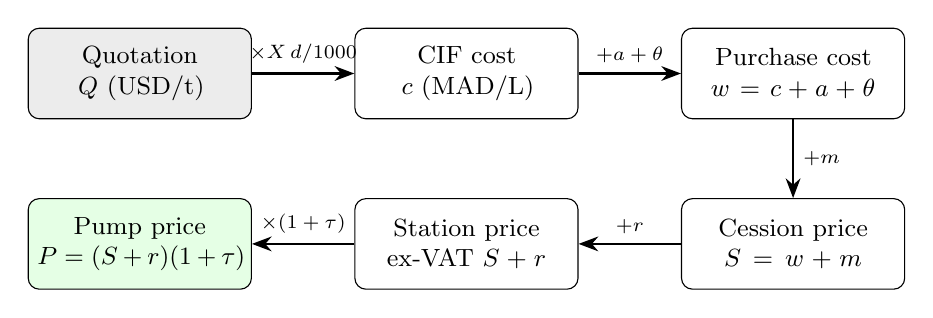
\begin{tikzpicture}[
  box/.style={draw, rounded corners, align=center, minimum height=1.15cm, text width=2.6cm, font=\small},
  arr/.style={-{Stealth[length=2.5mm]}, thick},
  lab/.style={font=\scriptsize, align=center}]
  \node[box, fill=gray!15] (q) {Quotation\\ $Q$ (USD/t)};
  \node[box, right=13mm of q] (c) {CIF cost\\ $c$ (MAD/L)};
  \node[box, right=13mm of c] (w) {Purchase cost\\ $w=c+a+\theta$};
  \node[box, below=10mm of w] (s) {Cession price\\ $S=w+m$};
  \node[box, left=13mm of s] (e) {Station price\\ ex-VAT $S+r$};
  \node[box, left=13mm of e, fill=green!10] (p) {Pump price\\ $P=(S+r)(1+\tau)$};
  \draw[arr] (q)--(c) node[midway, above, lab]{$\times X\,d/1000$};
  \draw[arr] (c)--(w) node[midway, above, lab]{$+a+\theta$};
  \draw[arr] (w)--(s) node[midway, right, lab]{$+m$};
  \draw[arr] (s)--(e) node[midway, above, lab]{$+r$};
  \draw[arr] (e)--(p) node[midway, above, lab]{$\times(1+\tau)$};
\end{tikzpicture}
\caption{The price chain. $a$: approach costs (port, unloading, storage) not already in the CIF;
$\theta$: the TIC; $m$: distributor gross margin; $r$: station margin; $\tau=0.10$: VAT.}
\label{fig:chain}
\end{figure}

Figure~\ref{fig:chain} reads as three equations, for each product and each period:
\begin{align}
w &= c + a + \theta &&\text{purchase cost (cost to the distributor, incl.\ TIC, excl.\ VAT)}\label{eq:w}\\
S &= w + m &&\text{cession price (distributor to partner station, excl.\ VAT)}\label{eq:S}\\
P &= (S + r)\,(1+\tau) &&\text{pump price, incl.\ VAT}\label{eq:P}
\end{align}
Combined,
\begin{equation}\label{eq:build}
P = (1+\tau)\,\big(c + a + \theta + m + r\big).
\end{equation}

The two taxes behave very differently, and this drives most of what follows:
\begin{itemize}
\item The \textbf{TIC} $\theta$ is a \emph{fixed amount per litre}\tagS (about 2.42~MAD/L for gasoil
  and 3.76~MAD/L for SSP\tagS). It does not change when the world price changes.
\item \textbf{VAT} is a \emph{percentage} ($\tau=10\%$) applied to everything before it, including the TIC.
\end{itemize}

\begin{intuition}
A fixed tax is a fixed number of dirhams in every litre, whether fuel is cheap or dear. A
percentage tax grows with the price. At the pump you pay the product, then the fixed TIC on top,
then the percentage VAT on the sum.
\end{intuition}

\subsection{How the tax share moves}

VAT collected on a litre is $\tau\,(S+r) = \tau P/(1+\tau)$. Total tax is $\theta + \tau P/(1+\tau)$, so
\begin{equation}\label{eq:taxshare}
\text{tax share} \;=\; \frac{\theta}{P} + \frac{\tau}{1+\tau}.
\end{equation}
The second term is a constant, $0.1/1.1 = 9.09\%$. The first term falls as $P$ rises. So \emph{when fuel
gets more expensive, the tax \emph{share} falls, even though tax rates did not change}. Politicians citing
``taxes are 60\% of the price'' and ``taxes are a small part of the increase'' can both be right.

\begin{worked}{tax share}
Gasoil, $\theta=2.42$. At $P=10.87$: $2.42/10.87 + 0.0909 = 31.4\%$. At $P=15.00$ with the same $\theta$:
$2.42/15 + 0.0909 = 25.2\%$.
\end{worked}

\section{Checking the structure against the Competition Council}

The CC publishes averages for Q4~2025 (MAD/L)\tagV. We know $c$, $w$, $S$, $P$ and the TIC; the unknowns are
$a$ and $r$ and we can \emph{infer} them by rearranging the chain:
\begin{equation}\label{eq:inverse}
a = w - c - \theta,\qquad m = S - w,\qquad r = \frac{P}{1+\tau} - S .
\end{equation}

\begin{table}[h]
\centering
\begin{tabular}{lrr}
\toprule
& Gasoil & SSP \\
\midrule
CIF quotation $c$ (CC) & 5.59 & 5.12 \\
Purchase cost $w$ (CC) & 8.10 & 9.00 \\
Cession price $S$ (CC) & 9.38 & 11.06 \\
Pump price $P$ (CC) & 10.87 & 12.82 \\
TIC $\theta$ (press) & 2.42 & 3.76 \\
\midrule
Implied approach cost $a = w - c - \theta$ & 0.09 & 0.12 \\
Gross margin $m = S - w$ & 1.28 & 2.06 \\
\quad (CC weighted figure) & 1.23 & 1.85 \\
$P/(1+\tau)$ & 9.882 & 11.655 \\
Implied station margin $r$ & 0.50 & 0.59 \\
VAT amount & 0.99 & 1.17 \\
Tax share $(\theta+\mathrm{VAT})/P$ & 31.4\% & 38.4\% \\
\bottomrule
\end{tabular}
\caption{Competition Council Q4 2025 averages (rows above the rule) and what they imply
(rows below). TIC from press reports\tagS. The CC's own weighted gross margin differs slightly from the
simple difference of two averages because it is averaged across firms and periods.}
\label{tab:cc}
\end{table}

\begin{figure}[h]
\centering
\begin{tikzpicture}
\begin{axis}[
  ybar stacked, bar width=42pt, symbolic x coords={Gasoil,SSP}, xtick=data,
  ymin=0, ymax=14.5, ylabel={MAD per litre}, height=8.5cm, width=0.62\textwidth,
  enlarge x limits=0.55, legend style={at={(1.04,0.5)},anchor=west,font=\small},
  legend cell align=left, area legend]
\addplot+[fill=blue!55,draw=none]  table[x=product,y=cif]{generated/stack.dat};
\addlegendentry{CIF quotation $c$}
\addplot+[fill=gray!55,draw=none]  table[x=product,y=approach]{generated/stack.dat};
\addlegendentry{approach $a$ (implied)}
\addplot+[fill=orange!70,draw=none] table[x=product,y=tic]{generated/stack.dat};
\addlegendentry{TIC $\theta$}
\addplot+[fill=red!60,draw=none]  table[x=product,y=gross]{generated/stack.dat};
\addlegendentry{distributor margin $m$}
\addplot+[fill=purple!55,draw=none] table[x=product,y=station]{generated/stack.dat};
\addlegendentry{station margin $r$ (implied)}
\addplot+[fill=green!45!black,draw=none] table[x=product,y=vat]{generated/stack.dat};
\addlegendentry{VAT}
\end{axis}
\end{tikzpicture}
\caption{What a litre of Moroccan gasoil and SSP was made of in Q4 2025, using the CC averages and the inverse
relations~\eqref{eq:inverse}.}
\label{fig:stack}
\end{figure}

Three consistency checks give confidence in the structure:
\begin{enumerate}
\item The implied approach costs are small and positive (0.09 and 0.12~MAD/L), as expected when the CIF already
  contains freight and insurance.
\item The implied tax shares (31.4\% and 38.4\%) match the shares the CC reports for Q4~2024 (31\% and 38\%)\tagV.
  That supports both the TIC amounts and the rule that VAT applies on top of the TIC.
\item The implied station margins (about 0.50--0.60~MAD/L) are plausible for retail.
\end{enumerate}

\begin{warning}
Two caveats. First, this checks that the chain is \emph{arithmetically consistent} with the CC tables, not that the
CC's CIF equals what distributors really paid. Second, we read ``HT'' (excl.\ taxes) in the CC tables as
\emph{excluding VAT but including the TIC}\tagQ. The reason: the gap between CIF and purchase cost (2.51~MAD/L for gasoil) is almost exactly the
TIC (2.42). If ``HT'' also excluded the TIC, that gap would have to be approach cost alone, which is implausibly large. Task 1.1 of the
plan is to confirm this in the CC methodology.

A subtler point: the CC's purchase cost is a \emph{book} cost that reflects stock held (Section~\ref{sec:inventory}), so the implied
$a$ in~\eqref{eq:inverse} mixes true approach costs with inventory gains or losses over the quarter. Over a quarter with small price moves
this is small; over a volatile quarter it need not be.
\end{warning}

\section{The VAT trap in pass-through ratios}\label{sec:vat}

Differentiate~\eqref{eq:build} with respect to the CIF cost, holding $a,\theta,m,r$ fixed:
\begin{equation}\label{eq:dPdc}
\frac{\partial P}{\partial c} = 1+\tau = 1.10 .
\end{equation}

\begin{keyidea}
A distributor who passes a cost change straight through, leaving its margins alone, raises the pump price by
\emph{1.10 times} the change in CIF, not by 1.0 times. Any ratio ``pump-price change over CIF change''
therefore reads 110\% for a perfect pass-through if the pump price includes VAT and the CIF does not.
\end{keyidea}

Define two measures for a cost change $\Delta c$ and pump change $\Delta P$:
\begin{equation}
\PT^{\mathrm{raw}} = \frac{\Delta P}{\Delta c},\qquad
\PT^{\mathrm{adj}} = \frac{\Delta P}{(1+\tau)\,\Delta c} = \frac{\PT^{\mathrm{raw}}}{1.10}.
\end{equation}
The CC's reported rates for the early-March 2026 episode (diesel 69.5\%, gasoline above 100\%)\tagS match $\PT^{\mathrm{raw}}$ if the CC divides
the (VAT-inclusive) pump change by the (VAT-free) CIF change\tagQ:

\begin{table}[h]
\centering
\begin{tabular}{lrrrr}
\toprule
& $\Delta c$ & $\Delta P$ & $\mathrm{PT}^{\mathrm{raw}}$ & $\mathrm{PT}^{\mathrm{adj}}$ \\
\midrule
Diesel & +2.92 & +2.03 & 69.5\% & 63.2\% \\
Gasoline & +1.26 & +1.43 & 113.5\% & 103.2\% \\
\bottomrule
\end{tabular}
\caption{Early-March 2026 episode as reported\tagS, raw and VAT-adjusted.}
\end{table}

If the CC does divide this way, the diesel rate is about 63\% rather than 69.5\%, and gasoline is roughly complete pass-through (103\%)
rather than ``more than complete'' (113\%). This does not say the CC is wrong, only that two readers could draw different conclusions
from the same pair of numbers. Our tool should display both and explain the difference.

\subsection{The inversion puzzle, as arithmetic}\label{sec:puzzle}

Take two products with the same margins and approach costs, differing in $c$ and $\theta$. From~\eqref{eq:build},
\[
P_{\text{gasoil}} - P_{\text{SSP}} = (1+\tau)\big[(c_{\text{gasoil}} - c_{\text{SSP}}) + (\theta_{\text{gasoil}}-\theta_{\text{SSP}})\big].
\]
With $\theta_{\text{gasoil}}-\theta_{\text{SSP}} = 2.42 - 3.76 = -1.34$ and a pump gap of about $+1.40$~MAD/L (press, 1~Nov)\tagS:
\[
c_{\text{gasoil}} - c_{\text{SSP}} = \frac{1.40}{1.10} + 1.34 \approx 2.61~\MADL .
\]
In Q4~2025 the gap in CIF was $5.59 - 5.12 = 0.47$~MAD/L\tagV. The inversion therefore predicts that diesel quotations have
moved about 2~MAD/L above gasoline quotations relative to Q4~2025. That is directly testable against refined-product quotations; if it
\emph{fails}, the explanation must lie in margins or in how prices are set, which is exactly the interesting finding.

% =============================================================================
\part{Time and inventories}

\section{Prices are fixed for a fortnight, costs move every day}\label{sec:window}

World quotations change daily; the pump price is fixed between revisions on the 1st and 16th. Which cost should we compare a
pump price with?

\begin{definition}[Window-averaged cost]
For revision $t$, let $s_t$ be the last day of the observation window. Then
\begin{equation}
\bar c_t = \sum_{j=0}^{J} \omega_j\, c_{s_t - j},\qquad \omega_j\ge 0,\ \sum_j \omega_j = 1 .
\end{equation}
\end{definition}
The window length $J$, the lag between window end and revision, and the weights $\omega_j$ are not known to us. A fortnightly average
ending a day or two before the revision is a natural starting guess; the old administered formula used a fortnightly average\tagQ. We
\emph{estimate} the window by trying a grid of choices and keeping those that predict pump-price changes best out of sample, and report the
whole surface rather than just its maximum.

\begin{intuition}
Suppose distributors set the new price using the average of the last 15 days, but we compare it with the quotation on the revision day. We
are then using a noisy stand-in for the true cost. Noise in the explanatory variable always pulls the estimated response towards zero.
\end{intuition}

Formally, if we observe $\tilde x = x + e$ with noise variance $\sigma_e^2$ and true signal variance $\sigma_x^2$, a regression of $y=\beta x+\varepsilon$ on
$\tilde x$ converges to
\begin{equation}\label{eq:attenuation}
\hat\beta \;\to\; \beta\,\frac{\sigma_x^2}{\sigma_x^2+\sigma_e^2}\;<\;\beta .
\end{equation}
The consequence for our subject is serious: \emph{a mis-timed cost variable can make a market that passes through everything look as if
it passes through only part.} This is why Section~\ref{sec:window} comes before any claim about pass-through.

\section{Inventories: why a delay is not an accusation}\label{sec:inventory}

Distributors hold stock bought earlier at older prices. The legal minimum is 60 days of consumption\tagS. The CC's purchase cost is a
weighted average that includes stock variations\tagV, so it reacts to quotation changes with a delay.

\subsection{A minimal model: weighted-average cost}

Let $R_t = c_t + a_t + \theta$ be the \emph{replacement cost} (what rebuying today costs). Let $A_t$ be the \emph{book cost} (the weighted average
of what is in stock). In each fortnight a share $\lambda$ of the stock is replaced:
\begin{equation}\label{eq:wac}
A_t = (1-\lambda)\,A_{t-1} + \lambda\,R_t \;=\; \lambda\sum_{k\ge 0}(1-\lambda)^k R_{t-k}.
\end{equation}
So the book cost is an \emph{exponentially weighted average} of past replacement costs. Its average delay is $(1-\lambda)/\lambda$ fortnights. If the stock
covers $D$ days, then roughly $\lambda\approx 15/(D+15)$ and the mean delay is $D/15$ fortnights: 30 days of stock means a two-fortnight lag.

Two margins follow, and confusing them is a classic source of misunderstanding:
\begin{align}
\text{replacement-cost margin: } m^R_t &= S_t - R_t, \\
\text{book-cost margin: } m^H_t &= S_t - A_t, \\
\text{inventory gain: } m^H_t - m^R_t &= R_t - A_t .
\end{align}
When costs have been rising, $R_t > A_t$: stock is cheaper than rebuying, so the book margin exceeds the replacement margin (a holding gain).
When costs have been falling, the reverse holds.

\subsection{A toy experiment with three pricing rules}

Let the CIF cost move as $c=6$ for fortnights $0$--$3$, drop to $5$ at fortnights $4$--$7$, and return to $6$ at fortnights $8$--$11$
(a 1~MAD/L swing). Take $a=0.10$, $\theta=2.42$, a target margin of $1.20$~MAD/L and $\lambda=1/3$. Three distributors follow different rules:
\begin{description}[leftmargin=2em]
\item[Rule 1] $S^{(1)}_t = R_t + 1.20$: margin over \emph{replacement} cost.
\item[Rule 2] $S^{(2)}_t = A_t + 1.20$: margin over \emph{book} cost (``cost-plus'' on what is in the tank).
\item[Rule 3] $S^{(3)}_t = \max(R_t, A_t) + 1.20$: margin over the \emph{dearer} of the two costs.
\end{description}

\begin{table}[h]
\centering
\begin{tabular}{rrrrrr}
\toprule
$t$ & $R_t$ & $A_t$ & $S^{(1)}_t$ & $S^{(2)}_t$ & $S^{(3)}_t$ \\
\midrule
0 & 8.52 & 8.52 & 9.72 & 9.72 & 9.72 \\
1 & 8.52 & 8.52 & 9.72 & 9.72 & 9.72 \\
2 & 8.52 & 8.52 & 9.72 & 9.72 & 9.72 \\
3 & 8.52 & 8.52 & 9.72 & 9.72 & 9.72 \\
4 & 7.52 & 8.19 & 8.72 & 9.39 & 9.39 \\
5 & 7.52 & 7.96 & 8.72 & 9.16 & 9.16 \\
6 & 7.52 & 7.82 & 8.72 & 9.02 & 9.02 \\
7 & 7.52 & 7.72 & 8.72 & 8.92 & 8.92 \\
8 & 8.52 & 7.99 & 9.72 & 9.19 & 9.72 \\
9 & 8.52 & 8.16 & 9.72 & 9.36 & 9.72 \\
10 & 8.52 & 8.28 & 9.72 & 9.48 & 9.72 \\
11 & 8.52 & 8.36 & 9.72 & 9.56 & 9.72 \\
\bottomrule
\end{tabular}
\caption{Replacement cost $R_t$, book cost $A_t$ and cession prices under the three rules (MAD/L).}
\end{table}

\begin{figure}[h]
\centering
\begin{tikzpicture}
\begin{axis}[width=0.9\textwidth,height=7cm,xlabel={fortnight $t$},ylabel={MAD per litre},
  xmin=0,xmax=11,legend style={at={(0.5,-0.22)},anchor=north,legend columns=2,font=\small},
  grid=major,grid style={gray!25}]
\addplot[black,dashed,thick]   table[x=t,y=R]{generated/inventory.dat};   \addlegendentry{replacement cost $R_t$}
\addplot[gray,dotted,thick]    table[x=t,y=A]{generated/inventory.dat};   \addlegendentry{book cost $A_t$}
\addplot[blue,thick,mark=*,mark size=1.5pt]   table[x=t,y=S1]{generated/inventory.dat}; \addlegendentry{rule 1 price}
\addplot[orange!85!black,thick,mark=square*,mark size=1.5pt] table[x=t,y=S2]{generated/inventory.dat}; \addlegendentry{rule 2 price}
\addplot[red!70!black,thick,mark=triangle*,mark size=2pt]   table[x=t,y=S3]{generated/inventory.dat}; \addlegendentry{rule 3 price}
\end{axis}
\end{tikzpicture}
\caption{The three pricing rules in the toy model. Rule~2 lags both the fall and the rise; Rule~3 follows
rises immediately but falls only with the book cost (rule~3 and rule~2 coincide during the fall).}
\label{fig:inventory}
\end{figure}

To summarise how far each rule's price sits above the replacement-cost benchmark ($R_t + 1.20$), add up the differences over the fall window and
over the rise window:

\begin{table}[h]
\centering
\begin{tabular}{lrr}
\toprule
Pricing rule & Over the fall (t=4--7) & Over the rise (t=8--11) \\
\midrule
Replacement cost-plus & +0.00 & +0.00 \\
Book cost-plus & +1.60 & -1.29 \\
Dearer of the two & +1.60 & +0.00 \\
\bottomrule
\end{tabular}
\caption{Cumulative departure of the cession price from the replacement-cost-plus benchmark, MAD/L summed over four fortnights.}
\end{table}

\begin{table}[h]
\centering
\begin{tabular}{lrr}
\toprule
Pricing rule & mean replacement margin $\bar m^{R}$ & mean book margin $\bar m^{H}$ \\
\midrule
Replacement cost-plus & 1.20 & 1.17 \\
Book cost-plus & 1.23 & 1.20 \\
Dearer of the two & 1.33 & 1.31 \\
\bottomrule
\end{tabular}
\caption{Average margins over the whole 12-fortnight cycle (MAD/L).}
\end{table}

\begin{keyidea}
\begin{enumerate}[leftmargin=1.5em]
\item \textbf{A lag is not an asymmetry.} Rule~2 is slow in both directions: over-priced relative to replacement cost during the fall, under-priced
  during the rise. A distributor that merely adds a constant margin to its book cost looks, on a replacement-cost benchmark, like a villain in the fall
  and a hero in the rise. Its \emph{book} margin is constant at 1.20.
\item \textbf{An asymmetry needs a rule that treats the two directions differently.} Rule~3 behaves like Rule~1 when costs rise and
  like Rule~2 when they fall: ``rockets and feathers.'' It earns about 0.13~MAD/L more than the benchmark on average, but there is no
  statistical way, from prices alone, to tell whether that rule comes from prudence (protecting against restocking at higher cost), search frictions
  or market power.
\item \textbf{So we need two benchmarks and the stage-by-stage view} (Section~\ref{sec:stages}): replacement cost versus book cost,
  and each link of the chain separately.
\end{enumerate}
\end{keyidea}

\begin{warning}
The three rules are illustrations. Nothing here says any distributor uses one. The point is to see that the same observed pump-price pattern can
come from very different behaviour, which is why the project's wording rules forbid accusations.
\end{warning}

% =============================================================================
\part{Pass-through and asymmetry}

\section{Definitions}

Work with additive, tax-free quantities, because the structure~\eqref{eq:build} is additive:
\begin{itemize}
\item $\bar c_t$: window-averaged cost (Section~\ref{sec:window}), MAD/L.
\item $p_t = P_t/(1+\tau) - \theta$: the \emph{net-of-tax pump price}.
\item $\mu_t = p_t - \bar c_t = a + m_t + r_t$: the \emph{margin gap}, everything between cost and tax-free price.
\item $\Delta x_t = x_t - x_{t-1}$ (change since the previous fortnight), and
  $\Delta\bar c^{+}_t = \max(\Delta\bar c_t,0)$, $\Delta\bar c^{-}_t=\min(\Delta\bar c_t,0)$ (rises and falls separately).
\end{itemize}

\begin{definition}[Pass-through]
If a cost change $\Delta\bar c$ moves the net-of-tax pump price by $B\,\Delta\bar c$ after $h$ fortnights, then $B_h$ is the cumulative pass-through at horizon $h$.
Pass-through is \emph{complete} when $B_h\to 1$.
\end{definition}

\begin{definition}[Asymmetric price transmission]
\emph{Speed (time) asymmetry}: rises are passed on faster than falls. \emph{Magnitude (size) asymmetry}: rises are passed on in larger amounts. The
pattern is nicknamed ``rockets and feathers'' after Bacon (1991)\cite{bac91}. In a classic US study, nearly all of a crude-oil rise reached the pump in four weeks while falls took about eight, and the asymmetry arose mostly between wholesale and
retail prices, not between crude and wholesale\tagV\cite{bcg97}.
\end{definition}

Candidate explanations are many: inventory valuation (Section~\ref{sec:inventory}), search costs, menu costs, and market power. A significant asymmetry is
\emph{evidence of a pattern}, not of intent.

\section{The model ladder}

We climb from simple to rich and stop when the next rung does not change the conclusions.

\subsection*{M0 --- Descriptive margins (no statistics)}
Plot $\mu_t$ with the CC-reported margins for comparison. Count fortnights where $\mu_t$ rises while $\bar c_t$ falls. It needs no econometrics and is easy to explain, so
it comes first.

\subsection*{M1 --- Symmetric distributed lag}
\begin{equation}\label{eq:m1}
\Delta p_t = \alpha + \sum_{k=0}^{K}\beta_k\,\Delta\bar c_{t-k} + \varepsilon_t .
\end{equation}
Today's price change responds to today's and the last $K$ cost changes. The cumulative pass-through is $B_h=\sum_{k=0}^h\beta_k$; the mean adjustment lag is
$\bar k = \sum_k k\beta_k/\sum_k\beta_k$ fortnights. If the same response applies to rises and falls the model is \emph{symmetric}.

\subsection*{M2 --- Asymmetric distributed lag}
\begin{equation}\label{eq:m2}
\Delta p_t = \alpha + \sum_{k=0}^{K}\Big(\beta^{+}_k\,\Delta\bar c^{+}_{t-k} + \beta^{-}_k\,\Delta\bar c^{-}_{t-k}\Big) + \varepsilon_t .
\end{equation}
Define cumulative responses $B^{+}_h=\sum_{k\le h}\beta^{+}_k$ and $B^{-}_h=\sum_{k\le h}\beta^{-}_k$ and the \textbf{rocket--feather gap}
\begin{equation}
\AI_h = B^{+}_h - B^{-}_h .
\end{equation}
Under symmetry $\AI_h = 0$ for every $h$. This is the design of Borenstein, Cameron and Gilbert\cite{bcg97}. We test $H_0:\AI_h=0$ with a Wald/$t$ test using
HAC standard errors (Section~\ref{sec:hac}).

\subsection*{M3 --- The margin form (the most readable)}
Since $\Delta\mu_t = \Delta p_t - \Delta\bar c_t$, substituting~\eqref{eq:m2} gives the same model with new coefficients,
\begin{equation}\label{eq:m3}
\Delta\mu_t = \alpha + \sum_{k=0}^{K}\Big(\delta^{+}_k\,\Delta\bar c^{+}_{t-k} + \delta^{-}_k\,\Delta\bar c^{-}_{t-k}\Big) + \varepsilon_t,\qquad
\delta_k=\beta_k - \ind[k=0] .
\end{equation}
With complete, immediate pass-through every $\delta$ is zero. Cost rises squeeze the margin ($\delta^{+}<0$); cost falls widen it
($\delta^{-}<0$ because $\Delta\bar c^{-}<0$). ``Margins widen when costs fall'' is what the public debate is about, and M3 turns it into one coefficient to display.

\subsection*{M4 --- Error correction}
Prices are pulled back to a long-run relation like a rubber band. Step 1: estimate $p_t = a_0 + b\,\bar c_t + u_t$ (the deviation $u_t$ is the margin
relative to its norm). Step 2:
\begin{equation}\label{eq:m4}
\Delta p_t = \sum_k\Big(\beta^{+}_k\Delta\bar c^{+}_{t-k}+\beta^{-}_k\Delta\bar c^{-}_{t-k}\Big)+\gamma^{+}u^{+}_{t-1}+\gamma^{-}u^{-}_{t-1}+\sum_j\phi_j\Delta p_{t-j}+\varepsilon_t,
\end{equation}
where $u^{+}=\max(u,0)$ means the price is above its long-run level (margin fat) and $u^{-}=\min(u,0)$ means it is below (margin thin). Both $\gamma$ are
expected to be negative. ``Rockets and feathers'' corresponds to $|\gamma^{-}|>|\gamma^{+}|$: thin margins are repaired faster than fat margins are competed away.
If a deviation shrinks by the factor $\rho=1+\gamma$ each fortnight, then $u_{t+h}=\rho^h u_t$ and the \emph{half-life} $h^\ast$ satisfies $\rho^{h^\ast}=1/2$:
\begin{equation}\label{eq:halflife}
h^\ast = \frac{\ln 0.5}{\ln(1+\gamma)} .
\end{equation}

\begin{table}[h]
\centering
\begin{tabular}{rr}
\toprule
$\gamma$ & half-life (fortnights) \\
\midrule
-0.8 & 0.4 \\
-0.5 & 1.0 \\
-0.3 & 1.9 \\
-0.2 & 3.1 \\
-0.1 & 6.6 \\
\bottomrule
\end{tabular}
\caption{Half-life of a margin deviation for different adjustment speeds $\gamma$.}
\end{table}

M4 needs the pump price and the cost to be \emph{cointegrated} (Section~\ref{sec:coint}).

\subsection*{M5 and M6 --- Nonlinear ARDL and thresholds}
NARDL builds the partial sums $c^{\pm}_t=\sum_{j\le t}\Delta c^{\pm}_j$ and lets the long-run multipliers differ for rises and falls\cite{syg14}. Threshold models let the adjustment depend on the \emph{size}
of the margin, e.g.\ nothing happens inside a band and adjustment starts only outside it\cite{qz}. These are used only if M2--M4 leave something unexplained.

\section{A simulation you can reproduce}\label{sec:sim}

Theory is easier to trust once you have seen it work on data where the truth is known. We simulate 240 fortnights (about ten years). Cost changes are drawn from a
heavy-tailed distribution with standard deviation 0.30~MAD/L. The pump price follows the asymmetric lag structure of~\eqref{eq:m2} with $K=4$:
\[
\beta^{+}=(0.70,\,0.30,\,0,\,0,\,0),\qquad \beta^{-}=(0.30,\,0.30,\,0.20,\,0.10,\,0.10),
\]
plus small noise. Both sum to 1, so pass-through is eventually complete in both directions, but rises are fully passed on within two fortnights while falls take five.

\begin{figure}[h]
\centering
\begin{tikzpicture}
\begin{axis}[width=0.72\textwidth,height=7cm,xlabel={cost change $\Delta\bar c_t$ (MAD/L)},
  ylabel={pump price change $\Delta p_t$ (MAD/L)},grid=major,grid style={gray!25}]
\addplot[only marks,mark=*,mark size=1.2pt,blue!60,opacity=0.7] table[x=dc,y=dp]{generated/sim_scatter.dat};
\end{axis}
\end{tikzpicture}
\caption{Simulated data (first 120 fortnights). Same-fortnight cost and price changes are only loosely related because response is spread over several fortnights and differs for rises and falls; the scatter alone hides the asymmetry.}
\end{figure}

\begin{table}[h]
\centering
\begin{tabular}{rrrrrr}
\toprule
lag $k$ & true $\beta^{+}_k$ & est. $\hat\beta^{+}_k$ (s.e.) & true $\beta^{-}_k$ & est. $\hat\beta^{-}_k$ (s.e.) & \\
\midrule
0 & 0.70 & 0.67 (0.03) & 0.30 & 0.27 (0.03) & \\
1 & 0.30 & 0.32 (0.03) & 0.30 & 0.29 (0.04) & \\
2 & 0.00 & 0.01 (0.02) & 0.20 & 0.20 (0.03) & \\
3 & 0.00 & 0.02 (0.03) & 0.10 & 0.12 (0.03) & \\
4 & 0.00 & 0.05 (0.02) & 0.10 & 0.12 (0.03) & \\
\bottomrule
\end{tabular}
\caption{True and estimated lag coefficients from OLS on the simulated sample; Newey--West standard errors in parentheses.}
\end{table}

\begin{table}[h]
\centering
\begin{tabular}{rrrrr}
\toprule
horizon $h$ & $\hat B^{+}_h$ & $\hat B^{-}_h$ & gap $\hat{\mathrm{AI}}_h$ & $p$-value \\
\midrule
0 & 0.67 & 0.27 & +0.40 & 0.000 \\
1 & 0.99 & 0.56 & +0.43 & 0.000 \\
2 & 1.00 & 0.76 & +0.24 & 0.009 \\
3 & 1.01 & 0.88 & +0.13 & 0.202 \\
4 & 1.06 & 0.99 & +0.07 & 0.562 \\
\bottomrule
\end{tabular}
\caption{Cumulative rocket--feather gap $\hat{\AI}_h = \hat B^{+}_h-\hat B^{-}_h$ and its $p$-value. The true gaps are $0.4,\,0.4,\,0.2,\,0.1,\,0$ for $h=0,\dots,4$.}
\end{table}

\begin{figure}[h]
\centering
\begin{tikzpicture}
\begin{axis}[width=0.75\textwidth,height=7cm,xlabel={horizon $h$ (fortnights)},
  ylabel={cumulative pass-through $B_h$},xmin=0,xmax=4,ymin=0,ymax=1.15,xtick={0,1,2,3,4},
  grid=major,grid style={gray!25},legend style={at={(0.97,0.05)},anchor=south east,font=\small}]
\addplot[blue,thick,mark=*]        table[x=h,y=cum_up]{generated/sim_cumulative.dat};  \addlegendentry{rises, estimated}
\addplot[blue,dashed]              table[x=h,y=true_up]{generated/sim_cumulative.dat}; \addlegendentry{rises, true}
\addplot[red!70!black,thick,mark=square*] table[x=h,y=cum_dn]{generated/sim_cumulative.dat};  \addlegendentry{falls, estimated}
\addplot[red!70!black,dashed]      table[x=h,y=true_dn]{generated/sim_cumulative.dat}; \addlegendentry{falls, true}
\end{axis}
\end{tikzpicture}
\caption{Cumulative pass-through of rises and falls: the ``rockets and feathers'' picture, recovered from simulated data.}
\end{figure}

The estimates are close to the truth and the test detects the early-horizon gap. By $h=3$ and $h=4$ the true gap is small (0.1 and 0) and the test, rightly, does not reject.

\subsection{How often would the test be right? (size and power)}

A single run proves little. We repeat the experiment 1000 times for three sample sizes and record how often the test of $H_0:B^{+}_1=B^{-}_1$ rejects at the 5\% level,
once when the world is symmetric (a good test rejects about 5\% of the time: its \emph{size}) and once when it is asymmetric as above (a good test rejects often: its
\emph{power}).

\begin{table}[h]
\centering
\begin{tabular}{rrr}
\toprule
sample size $n$ & rejection rate if symmetric (size) & rejection rate if asymmetric (power) \\
\midrule
60 & 12.7\% & 74.5\% \\
120 & 10.2\% & 94.1\% \\
240 & 7.9\% & 100.0\% \\
\bottomrule
\end{tabular}
\caption{Monte Carlo size and power of the HAC test of $H_0:B^{+}_1=B^{-}_1$ (nominal level 5\%, 1000 repetitions).}
\end{table}

\begin{warning}
With only 60 observations (roughly what one regime between structural breaks would give us) a perfectly symmetric market is flagged as asymmetric about
1~time in 8, not 1~in 20. The standard errors are too optimistic in small samples. Remedies we will use: bootstrap or small-sample corrections, pooling gasoil and SSP, requiring
the result to hold across specifications, and writing hypotheses down \emph{before} looking at the data (pre-registration).
\end{warning}

\section{Where does the delay arise? Stage by stage}\label{sec:stages}

Borenstein et al.\ located the US asymmetry by testing each link of the chain separately\cite{bcg97}. Morocco's chain is only partly observable, but the CC series let us do the same:

\begin{center}
\small
\begin{tabular}{p{4.0cm}p{3.7cm}p{5.0cm}}
\toprule
Link & Observable via & Where a delay could come from \\
\midrule
Quotation $\to$ purchase cost & CC (quarterly) & Inventory valuation (Section~\ref{sec:inventory}) \\
Purchase cost $\to$ cession price & CC (quarterly) & The distributor's pricing decision \\
Cession price $\to$ pump price & CC and press prices & Station margin, contracts, rounding \\
\bottomrule
\end{tabular}
\end{center}

If the delay is already in the first link it is mostly an accounting artefact; if it arises in the second it is a pricing choice. The CC's Q4~2025 report offers a gasoil example of the second kind: purchase cost rose by 0.22~MAD/L while the cession price fell by 0.29,
a gap of 0.51~MAD/L that the CC reads as partial absorption by distributors\tagV.

% =============================================================================
\part{The statistics you need, in plain language}

\section{Why not just run a regression? Stationarity and cointegration}\label{sec:coint}

\begin{intuition}
A \emph{random walk} wanders without a fixed mean, like a drunk walking in a field. Two drunks walking independently each wander away from where they started. Plot them
together and they often seem to move in step for long stretches. Regress one on the other and the regression will usually find a ``significant relationship'' that is pure coincidence.
Prices are typically like this. If one drunk walks a dog on a leash, however, the two paths stay close: they are \emph{cointegrated}.
\end{intuition}

\begin{table}[h]
\centering
\begin{tabular}{lr}
\toprule
Independent random walks, $n=240$, 2000 repetitions & \\
\midrule
Share of repetitions where the slope looks ``significant'' at 5\% & 85\% \\
Average $R^2$ & 0.24 \\
\bottomrule
\end{tabular}
\caption{The danger of regressing wandering series on each other. The two series are independent by construction, yet the usual test finds a ``relationship'' most of the time.}
\end{table}

Fuel prices and costs, in levels, behave like random walks. This yields a procedure:

\begin{enumerate}[leftmargin=2em]
\item \textbf{Unit-root tests} (ADF, KPSS; Zivot--Andrews if a break is plausible) tell whether a series wanders (it is \emph{integrated}, I(1)) or hovers around a fixed level (\emph{stationary}, I(0)). We expect $p_t$ and $\bar c_t$ to be I(1)
  and the margin gap $\mu_t$ to be I(0) if the market passes costs through completely in the long run.
\item \textbf{Cointegration} (Engle--Granger two-step; Johansen for both products together; Gregory--Hansen if the relation shifts) tests whether $p_t - b\,\bar c_t$ is stationary, i.e.\ whether there is a leash. If yes, error-correction models such as M4 are valid. If not, work with changes (M1--M3) only.
\item \textbf{Report} the unit-root and cointegration results alongside any pass-through estimate, so a reader can see the model was allowed.
\end{enumerate}

\section{Structural breaks}

The relation between prices and costs need not stay the same over ten years. Candidate break points are the liberalisation (1~Dec 2015), the 2022 price shock, the CC settlements (23~Nov 2023) and the Middle East shock of March 2026\tagS. Two reasons to take breaks seriously:
\begin{itemize}
\item Pooling data across a break averages two different regimes into a relationship that holds in neither.
\item Tests of asymmetry are known to reject too often when breaks are ignored\cite{robust}: a shift in behaviour can masquerade as asymmetry.
\end{itemize}
The method is: test for breaks (Bai--Perron), report break dates and uncertainty, estimate by regime. The cost is sample size, which is the next problem.

\section{Autocorrelation, overlap and HAC standard errors}\label{sec:hac}

Ordinary regression software assumes each error is independent of the others. In price data the error today is related to the error yesterday, so the software
reports standard errors that are too small and tests that reject too easily. \emph{HAC} (heteroskedasticity- and autocorrelation-consistent, or Newey--West) standard errors correct this by letting nearby errors be related, at the cost of needing a choice of how many lags to allow. We used four lags in
Section~\ref{sec:sim}. As the Monte Carlo showed, the correction is imperfect in small samples. Overlapping windows (a window longer than 15 days) create autocorrelation by construction, which is one more reason to keep windows within a fortnight where we can.

\section{How much data do we really have?}

About 24 revisions a year since 2016 gives roughly 240 observations per product. Breaks split these into three or four regimes of 50 to 100 observations. That supports distributed-lag models with four to six lags and comparisons between two regimes. It does \emph{not} support rich nonlinear models, unless the two
products are pooled. The Monte Carlo results show what is detectable. The honest conclusion in many cases will be ``not enough data to tell'', and the product should be able to say so.

\begin{keyidea}
\textbf{The recipe.} (1) Describe margins and costs with plots (M0). (2) Estimate and validate the cost window. (3) Test for unit roots, cointegration and breaks. (4) Fit M1, then M2/M3, by regime, with HAC or bootstrap inference. (5) Use M4--M6 only if the data demand them. (6) Check each link of the chain. (7) Report results with intervals and the hypotheses fixed in advance.
\end{keyidea}

% =============================================================================
\part{Uncertainty}

\section{Why every gap is an interval}

True purchase costs, approach costs and station margins are unobserved. To say whether a pump price is ``high'', we need a reference price
\begin{equation}\label{eq:pstar}
P^{\ast} = (1+\tau)\big(c + \hat a + \theta + \bar m + \bar r\big),
\end{equation}
using estimated or assumed values for the approach cost $\hat a$ and reference margins $\bar m,\bar r$. The model-implied gap is $G = P - P^{\ast}$.

\begin{worked}{how wide is the band?}
Suppose we only know $a\in[0.05,0.20]$, $\bar m\in[1.00,1.50]$ and $\bar r\in[0.40,0.70]$ (reasonable ranges given Table~\ref{tab:cc}). The non-cost, non-tax part inside the bracket then lies in
$[1.45,\,2.40]$, so $P^{\ast}$ varies over
\[
1.10\times[1.45,\,2.40] = [1.60,\ 2.64]\ \text{MAD/L above the cost-plus-TIC part}.
\]
That is a band about 1.05~MAD/L wide from reference-margin uncertainty alone. \emph{A pump price within about half a dirham of our reference is indistinguishable from it.} A tool that shows a gap of 0.20~MAD/L as a single number overstates what we know.
\end{worked}

\section{Three ways to quantify uncertainty}

\subsection{Simulation (Monte Carlo)}
Draw the unknowns from plausible distributions, compute $G$ each time, and publish the 10th--90th percentile band and the share of draws with $G>0$:
\begin{enumerate}[leftmargin=2em]
\item Draw $d$ from a range around the textbook density, the approach cost as $a_t=\bar a+\eta_t$ with $\eta_t=\phi\eta_{t-1}+\nu_t$, the window length $J$, and reference margins $\bar m,\bar r$ from a justified distribution.
\item For each draw compute $\bar c_t$, $P^{\ast}_t$ and $G_t$.
\item Summarise the draws by their percentiles.
\end{enumerate}
Priors for $\bar a$ come from the CC-implied values (0.09 and 0.12~MAD/L in Q4~2025).

\subsection{A cost corridor (bounds, no probabilities)}
Define a lower and upper plausible cost, $c^{\text{low}}_t=c_t+a_{\min}$ and $c^{\text{high}}_t=c_t+a_{\max}+\text{premium}_{\max}$, with bounds justified by CC data. If the observed price exceeds the corridor plus the reference margins for several consecutive fortnights, the signal is robust even under the most generous cost assumptions.

\subsection{State-space estimation of a hidden margin}
To estimate a time-varying margin, treat the true margin gap as hidden and observe it with noise:
\begin{align}
y_t &= \mu_t + \epsilon_t, && y_t = P_t/(1+\tau)-\theta-\bar c_t \quad\text{(what we compute)}\\
\mu_t &= \mu_{t-1} + \zeta_t &&\text{(the hidden margin drifts slowly)}.
\end{align}
The CC quarterly margins serve as rare, accurate observations of $m_t+a_t+r_t$. A Kalman filter or Bayesian fit produces a smoothed margin path with credible intervals. We keep this for later; start with simulation.

\begin{intuition}
Reading a band: a narrow band far from zero is strong evidence; a wide band straddling zero means we cannot tell. Both are findings.
\end{intuition}

% =============================================================================
\part{Benchmarks, descriptive metrics and forecasting}

\section{Metrics that do not depend on our cost model}

These use pump prices alone, so they stay valid even if the cost model is challenged.
\begin{itemize}
\item \textbf{Net-of-tax benchmark against Europe.} Compute $N_t=P_t/(1+\tau)-\theta$ and compare it with the European Commission's Weekly Oil Bulletin ``prices without taxes'' (weighted EU average and countries such as Spain, Portugal and France), converted to MAD. Differences in retail costs, quality and blending rules mean the \emph{level} gap is not a margin; the informative part is how the gap \emph{changes}, especially around world-price falls.
\item \textbf{Synchronisation.} Let $B$ be the number of brands and
  \[
  \text{Sync}_t=\frac1B\sum_{b=1}^{B}\ind[\text{brand } b \text{ changes on revision date } t],
  \]
  together with the share of brands changing by the same amount (within 0.02~MAD).
\item \textbf{Cross-brand dispersion.} The standard deviation (or range) of pump prices across the main brands in one city in each fortnight.
\item \textbf{Direction agreement.} Count fortnights where the pump price rose while the cost window fell, and the reverse, with sizes.
\item \textbf{Event study.} For the November 2023 settlement fit $y_t=\alpha+\lambda t+\kappa D_t+\varepsilon_t$ with $D_t=\ind[t\ge \text{Nov 2023}]$ and $y_t\in\{\mu_t,\PT^{\text{adj}},\AI_4,\text{spread to EU}\}$. Other events coincide with the break, so $\hat\kappa$ is a \emph{description}, not a causal claim.
\end{itemize}

\section{Forecasting the next price revision}

A useful product feature and an independent check on the model: before the 1st and 16th, predict $\Delta P_{t+1}$ from the cost window already observed. Press reports often cite ``sources'' a day or two ahead\tagS, providing cheap out-of-sample tests.
\begin{itemize}
\item \textbf{Baselines:} no change; repeat the last change; last window's cost change times $(1+\tau)$.
\item \textbf{Model:} M1 or M2, re-estimated on an expanding window (rolling origin) so each forecast uses only past data.
\item \textbf{Scores:} mean absolute error (MAD/L), share of correct directions, share within 0.10~MAD/L.
\item \textbf{Intervals by conformal prediction:} hold out recent forecasts, take the absolute errors, and use their $\lceil(1-\alpha)(n+1)\rceil$-th smallest value $q$ as a half-width: $\hat{\Delta P}\pm q$. This gives coverage close to $1-\alpha$ without assuming a distribution.
\item \textbf{Rule:} publish only if the model beats the baseline out of sample.
\end{itemize}

% =============================================================================
\part{Interpretation and limits}

\section{What a gap does and does not mean}

\begin{center}
\small
\begin{tabular}{p{6.3cm}p{6.3cm}}
\toprule
We may say & We may not say \\
\midrule
``Model-implied margin gap of $x$ (band $y$--$z$) MAD/L.'' & ``Company X overcharged'' or ``profiteering''. \\
``Pass-through of the last fall was $x\%$ (adjusted for VAT), versus $y\%$ for the last rise.'' & ``Distributors are colluding.'' \\
``This pattern is consistent with several explanations, including stock valuation and pricing rules.'' & ``The gap proves ...'' \\
``CC-reported (Q4 2025): 1.23~MAD/L gross margin for gasoil.'' & Any CC figure presented as current. \\
\bottomrule
\end{tabular}
\end{center}

\begin{warning}
Stating that a named company acted unlawfully on the basis of a modelled gap exposes the project to being wrong in public. Four habits protect against that: intervals, the three-way labelling (observed, CC-reported, model-implied), pre-registered hypotheses, and publishing methods and code so others can check and challenge.
\end{warning}

\section{Open questions}

\begin{enumerate}[leftmargin=2em]
\item Which quotation, hub and window do distributors actually use? (Estimated, Section~\ref{sec:window}.)
\item Does the CC divide VAT-inclusive pump changes by VAT-free CIF changes? (Section~\ref{sec:vat}.)
\item Does ``HT'' in the CC tables include the TIC? (Section~3.)
\item Are fortnightly CC series published or only quarterly aggregates?
\item What was the legacy (pre-2015) price structure and its margins? It would supply a reference margin and a ``what the old formula would give'' benchmark.
\item Is there a public source for volumes and stock days by period, needed for $\lambda$?
\item What is the exact TIC per product and when did it change? (The press figures need confirming in the finance law.)
\end{enumerate}

% =============================================================================
\appendix

\section{Notation}

\begin{longtable}{>{$}l<{$}p{5.2cm}p{5.6cm}}
\toprule
\text{Symbol} & Meaning & Source or status \\
\midrule
\endhead
Q & quotation, USD per tonne & licensed (Platts); free proxies exist \\
X & exchange rate, MAD per USD & Bank Al-Maghrib reference rate \\
d & density, kg/L & assumed; calibrate \\
c & CIF cost, MAD/L, excl.\ TIC and VAT & derived by~\eqref{eq:unit} \\
\bar c_t & window-averaged CIF cost & estimated window \\
a & approach cost (port, unloading, storage) & latent; implied from CC \\
\theta & TIC (fixed per litre) & finance law; press figures \\
w & purchase cost (book), incl.\ TIC, excl.\ VAT & CC (quarterly average) \\
R_t & replacement cost $c_t+a_t+\theta$ & derived \\
A_t & book (weighted-average) cost & inventory model \\
\lambda & share of stock replaced per fortnight & $\approx 15/(D+15)$ \\
m & distributor gross margin & CC (quarterly average) \\
r & station (retail) margin & latent; implied \\
S & cession price, excl.\ VAT & CC \\
P & pump price, incl.\ VAT & press, stations \\
\tau & VAT rate, 0.10 & finance law \\
p_t & net-of-tax pump price $P_t/(1+\tau)-\theta$ & derived \\
\mu_t & margin gap $p_t-\bar c_t$ & derived \\
\PT & pass-through ratio (raw or VAT-adjusted) & Section~\ref{sec:vat} \\
B_h & cumulative pass-through at horizon $h$ & estimated \\
\AI_h & rocket--feather gap $B^{+}_h-B^{-}_h$ & estimated \\
\gamma^{\pm} & error-correction speeds & estimated \\
P^{\ast},\,G & reference price, model-implied gap & Eq.~\eqref{eq:pstar} \\
\bottomrule
\end{longtable}

\section{Derivations}

\subsection{Tax share, Eq.~\eqref{eq:taxshare}}
From~\eqref{eq:build}, $P/(1+\tau)=c+a+\theta+m+r$ is the pre-VAT price, so VAT $=\tau P/(1+\tau)$. Tax $=\theta+\tau P/(1+\tau)$. Dividing by $P$ gives $\theta/P+\tau/(1+\tau)$.

\subsection{VAT effect on pass-through, Eq.~\eqref{eq:dPdc}}
$P=(1+\tau)(c+a+\theta+m+r)$ is linear in $c$ with slope $1+\tau$. With $a,m,r,\theta$ fixed, $\Delta P=(1+\tau)\Delta c$. Hence $\PT^{\text{raw}}=\Delta P/\Delta c=1+\tau$ under full pass-through, and $\PT^{\text{adj}}=\PT^{\text{raw}}/(1+\tau)=1$.

\subsection{Weighted-average cost as an exponential average, Eq.~\eqref{eq:wac}}
Substitute $A_{t-1}=(1-\lambda)A_{t-2}+\lambda R_{t-1}$ repeatedly: $A_t=\lambda R_t+\lambda(1-\lambda)R_{t-1}+\lambda(1-\lambda)^2R_{t-2}+\dots$. The weights $\lambda(1-\lambda)^k$ sum to 1. Mean lag
$\sum_{k\ge0}k\lambda(1-\lambda)^k=(1-\lambda)/\lambda$. With $\lambda=15/(D+15)$ this is $D/15$.

\subsection{Half-life, Eq.~\eqref{eq:halflife}}
If $u_{t}=\rho\,u_{t-1}$ with $0<\rho<1$ then $u_{t+h}=\rho^hu_t$. The half-life $h^\ast$ solves $\rho^{h^\ast}=\tfrac12$, so $h^\ast=\ln(0.5)/\ln\rho$ with $\rho=1+\gamma$.

\subsection{Equivalence of M2 and M3, Eq.~\eqref{eq:m3}}
$\Delta\mu_t=\Delta p_t-\Delta\bar c_t$ and $\Delta\bar c_t=\Delta\bar c^{+}_t+\Delta\bar c^{-}_t$. Subtract $\Delta\bar c^{+}_t+\Delta\bar c^{-}_t$ from the right side of~\eqref{eq:m2}: only the lag-0 coefficients change, by $-1$ each. Also $\sum_k\delta^{\pm}_k=B^{\pm}_K-1$, so M3 coefficients sum to zero exactly when pass-through is complete.

\subsection{Attenuation, Eq.~\eqref{eq:attenuation}}
With $\tilde x=x+e$, $e$ independent of $x$ and $\varepsilon$: $\operatorname{plim}\hat\beta=\operatorname{Cov}(\tilde x,y)/\operatorname{Var}(\tilde x)=\beta\sigma_x^2/(\sigma_x^2+\sigma_e^2)$.

\section{Exercises}

\begin{enumerate}[label=\textbf{E\arabic*.},leftmargin=2.5em]
\item Convert a quotation of $650$~USD/t at $X=9.3$~MAD/USD for diesel ($d=0.84$) to MAD/L.
\item With $c=5.00$, $a=0.10$, $\theta=2.42$, $m=1.20$, $r=0.50$ and $\tau=0.10$, compute the pump price $P$.
\item Using the numbers of E2: what is the tax share? If $c$ rises by $1.00$ with everything else unchanged, by how much does $P$ rise? If $P$ in fact rises by $0.80$, compute $\PT^{\text{raw}}$ and $\PT^{\text{adj}}$.
\item A distributor carries 45 days of stock. Find $\lambda$ and the mean lag of its book cost in fortnights.
\item An error-correction model has $\gamma^{-}=-0.60$ and $\gamma^{+}=-0.20$. Compute both half-lives. What does this pattern suggest?
\item In M2 with $\beta^{+}=(0.7,0.3)$ find the M3 coefficients $\delta^{+}$.
\item In the Monte Carlo of Section~\ref{sec:sim}, why does the symmetric-world rejection rate fall as $n$ grows?
\item Suppose price changes are $+1.00$ when the cost window rises by 1.00 but only $-0.50$ for the first fortnight when it falls by 1.00. Is this enough to claim asymmetry? What else do you need?
\item Show that when $m$ and $r$ stay unchanged and $\theta$ is fixed, the \emph{net-of-tax} pump price satisfies $\Delta p=\Delta c$ under full pass-through (no 1.10 factor).
\end{enumerate}

\subsection*{Solutions}
\begin{enumerate}[label=\textbf{E\arabic*.},leftmargin=2.5em]
\item $650\times9.3\times0.84/1000=5.08$~MAD/L.
\item Pre-VAT price $=5.00+0.10+2.42+1.20+0.50=9.22$; $P=9.22\times1.10=10.14$.
\item Tax share $=2.42/10.142+0.0909=33.0\%$. A rise of $1.00$ in $c$ raises $P$ by $1.10$. If $\Delta P=0.80$: $\PT^{\text{raw}}=0.80$, $\PT^{\text{adj}}=0.80/1.10=72.7\%$.
\item $\lambda=15/(45+15)=0.25$; mean lag $=(1-0.25)/0.25=3$ fortnights ($=45/15$).
\item $h^{-}=\ln0.5/\ln0.40=0.76$ fortnights; $h^{+}=\ln0.5/\ln0.80=3.1$ fortnights. Thin margins are repaired about four times faster than fat ones are competed away: a ``rockets and feathers'' pattern in margin repair (still not proof of intent).
\item $\delta^{+}_0=0.7-1=-0.3$, $\delta^{+}_1=0.3$. They sum to zero: complete pass-through, with a temporary margin squeeze.
\item The HAC test is only correct asymptotically; the standard errors are biased downward in small samples and the bias shrinks as $n$ grows. Hence size approaches 5\%.
\item No. One fortnight's response is not the cumulative response; the second fortnight might close the gap. One needs the cumulative response at several horizons, standard errors, many episodes and the stage-by-stage check.
\item $p=P/(1+\tau)-\theta=c+a+m+r$; so $\Delta p=\Delta c$ when $a,m,r$ are fixed. This is why Section~\ref{sec:vat} measures pass-through on the net-of-tax price in the models of Part~IV.
\end{enumerate}

\section{Reproducing every number}

From the repository root:
\begin{verbatim}
pip install -e ".[dev]" statsmodels pandas
PYTHONPATH=src python3 docs/latex/make_examples.py
cd docs/latex && pdflatex mazoti_theory.tex && pdflatex mazoti_theory.tex
\end{verbatim}
The script writes tables and plot data to \texttt{docs/latex/generated/}. The simulation seeds are fixed, so results are identical on every run. The price-structure functions in \texttt{src/mazoti/pricing.py} are tested against the CC Q4~2025 figures (\texttt{pytest}).

% =============================================================================
\begin{thebibliography}{99}\small
\bibitem{bac91} R.~W.~Bacon (1991), ``Rockets and feathers: the asymmetric speed of adjustment of UK retail gasoline prices to cost changes'', \emph{Energy Economics}.
\bibitem{bcg97} S.~Borenstein, A.~C.~Cameron and R.~Gilbert (1997), ``Do gasoline prices respond asymmetrically to crude oil price changes?'', \emph{Quarterly Journal of Economics} 112(1), 305--339. \url{https://www.nber.org/papers/w4138}
\bibitem{mvct04} J.~Meyer and S.~von Cramon-Taubadel (2004), ``Asymmetric price transmission: a survey'', \emph{Journal of Agricultural Economics} 55(3), 581--611.
\bibitem{eck13} A.~Eckert (2013), ``Empirical studies of gasoline retailing: a guide to the literature'', \emph{Journal of Economic Surveys} 27(1), 140--166.
\bibitem{pel00} S.~Peltzman (2000), ``Prices rise faster than they fall'', \emph{Journal of Political Economy} 108(3), 466--502.
\bibitem{qz} F.~Qiu and W.~Zhang, ``Rockets and feathers in the oil and gasoline markets: in-depth analysis of three asymmetries'', working paper. \url{https://ageconsearch.umn.edu/record/344062/files/29388.pdf}
\bibitem{robust} ``La robustesse des tests de transmission asym\'etrique des prix en pr\'esence de changements structurels'', journal article (authors to be added). \href{https://www.econbiz.de/Record/la-robustesse-des-tests-de-transmission-asym%C3%A9trique-des-prix-en-pr%C3%A9sence-de-changements-structurels/10008604344}{econbiz record}
\bibitem{cc25} Conseil de la concurrence (Morocco), \emph{Reporting du 4\`eme trimestre et analyse des principaux indicateurs de performance au titre de l'ann\'ee 2025 des soci\'et\'es de distribution en gros de gasoil et d'essence}, 2026. \url{https://conseil-concurrence.ma}
\bibitem{syg14} Y.~Shin, B.~Yu and M.~Greenwood-Nimmo (2014), ``Modelling asymmetric cointegration and dynamic multipliers in a nonlinear ARDL framework''. \textsuperscript{\textcolor{red!70!black}{[?]}} \emph{recalled from memory; verify details before citing}
\end{thebibliography}

\subsection*{Methods references recalled from memory (verify before citing)}
\small
Engle and Granger (1987) on cointegration; Johansen (1991); Gregory and Hansen (1996); Granger and Lee (1989) and von Cramon-Taubadel and Loy (1996) on asymmetric error correction; Enders and Siklos (2001) on threshold cointegration; Zivot and Andrews (1992) on unit roots with a break; Bai and Perron (2003) on multiple breaks; Newey and West (1987) on HAC standard errors; Maskin and Tirole (1988) on Edgeworth price cycles; Hyndman and Athanasopoulos, \emph{Forecasting: Principles and Practice}, for rolling-origin evaluation.

\end{document}
